\chapter{Chapter XVII}

\begin{verse}
At eve, within yon studious nook,\\
I ope my brass-embossed book,\\
Portray'd with many a holy deed\\
Of martyrs crown'd with heavenly meed;\\
Then, as my taper waxes dim,\\
Chant, ere I sleep, my measured hymn.\\!
\rule{.7\textwidth}{.2pt}

Who but would cast his pomp away,\\
To take my staff and amice grey,\\
And to the world's tumultuous stage,\\
Prefer the peaceful Hermitage?\\!
\attrib{--Warton}
\end{verse}

\lettrine{N}{otwithstanding} the prescription of the genial hermit,
with which his
guest willingly complied, he found it no easy matter to bring the harp
to harmony.

``Methinks, holy father,'' said he, ``the instrument wants one string,
and the rest have been somewhat misused.''

``Ay, mark'st thou that?'' replied the hermit; ``that shows thee a
master of the craft. Wine and wassail,'' he added, gravely casting up
his eyes--``all the fault of wine and wassail!--I told Allan-a-Dale, the
northern minstrel, that he would damage the harp if he touched it after
the seventh cup, but he would not be controlled--Friend, I drink to thy
successful performance.''

So saying, he took off his cup with much gravity, at the same time
shaking his head at the intemperance of the Scottish harper.

The knight in the meantime, had brought the strings into some order, and
after a short prelude, asked his host whether he would choose a
``sirvente'' in the language of ``oc'', or a ``lai'' in the language of
``oui'', or a ``virelai'', or a ballad in the vulgar
English.\footnote{Note C. Minstrelsy. See page~\pageref{noteCXVII}.}

``A ballad, a ballad,'' said the hermit, ``against all the `ocs' and
`ouis' of France. Downright English am I, Sir Knight, and downright
English was my patron St Dunstan, and scorned `oc' and `oui', as he
would have scorned the parings of the devil's hoof--downright English
alone shall be sung in this cell.''

``I will assay, then,'' said the knight, ``a ballad composed by a Saxon
glee-man, whom I knew in Holy Land.''

It speedily appeared, that if the knight was not a complete master of
the minstrel art, his taste for it had at least been cultivated under
the best instructors. Art had taught him to soften the faults of a voice
which had little compass, and was naturally rough rather than mellow,
and, in short, had done all that culture can do in supplying natural
deficiencies. His performance, therefore, might have been termed very
respectable by abler judges than the hermit, especially as the knight
threw into the notes now a degree of spirit, and now of plaintive
enthusiasm, which gave force and energy to the verses which he sung.

\begin{verse}
\versetitle{The Crusader's Return.}

\flagverse{1.}
High deeds achieved of knightly fame,\\
From Palestine the champion came;\\
The cross upon his shoulders borne,\\
Battle and blast had dimm'd and torn.\\
Each dint upon his batter'd shield\\
Was token of a foughten field;\\
And thus, beneath his lady's bower,\\
He sung as fell the twilight hour:--\\!
\flagverse{2.}
``Joy to the fair!--thy knight behold,\\
Return'd from yonder land of gold;\\
No wealth he brings, nor wealth can need,\\
Save his good arms and battle-steed\\
His spurs, to dash against a foe,\\
His lance and sword to lay him low;\\
Such all the trophies of his toil,\\
Such--and the hope of Tekla's smile!\\!
\flagverse{3.}
``Joy to the fair! whose constant knight\\
Her favour fired to feats of might;\\
Unnoted shall she not remain,\\
Where meet the bright and noble train;\\
Minstrel shall sing and herald tell--\\
'Mark yonder maid of beauty well,\\
'Tis she for whose bright eyes were won\\
The listed field at Askalon!\\!
\flagverse{4.}
``\,`Note well her smile!--it edged the blade\\
Which fifty wives to widows made,\\
When, vain his strength and Mahound's spell,\\
Iconium's turban'd Soldan fell.\\
Seest thou her locks, whose sunny glow\\
Half shows, half shades, her neck of snow?\\
Twines not of them one golden thread,\\
But for its sake a Paynim bled.'\\!
\flagverse{5.}
``Joy to the fair!--my name unknown,\\
Each deed, and all its praise thine own\\
Then, oh! unbar this churlish gate,\\
The night dew falls, the hour is late.\\
Inured to Syria's glowing breath,\\
I feel the north breeze chill as death;\\
Let grateful love quell maiden shame,\\
And grant him bliss who brings thee fame.''\\!
\end{verse}

During this performance, the hermit demeaned himself much like a
first-rate critic of the present day at a new opera. He reclined back
upon his seat, with his eyes half shut; now, folding his hands and
twisting his thumbs, he seemed absorbed in attention, and anon,
balancing his expanded palms, he gently flourished them in time to the
music. At one or two favourite cadences, he threw in a little assistance
of his own, where the knight's voice seemed unable to carry the air so
high as his worshipful taste approved. When the song was ended, the
anchorite emphatically declared it a good one, and well sung.

``And yet,'' said he, ``I think my Saxon countrymen had herded long
enough with the Normans, to fall into the tone of their melancholy
ditties. What took the honest knight from home? or what could he expect
but to find his mistress agreeably engaged with a rival on his return,
and his serenade, as they call it, as little regarded as the
caterwauling of a cat in the gutter? Nevertheless, Sir Knight, I drink
this cup to thee, to the success of all true lovers--I fear you are
none,'' he added, on observing that the knight (whose brain began to be
heated with these repeated draughts) qualified his flagon from the water
pitcher.

``Why,'' said the knight, ``did you not tell me that this water was from
the well of your blessed patron, St Dunstan?''

``Ay, truly,'' said the hermit, ``and many a hundred of pagans did he
baptize there, but I never heard that he drank any of it. Every thing
should be put to its proper use in this world. St Dunstan knew, as well
as any one, the prerogatives of a jovial friar.''

And so saying, he reached the harp, and entertained his guest with the
following characteristic song, to a sort of derry-down chorus,
appropriate to an old English ditty.\footnote{It may be proper to remind
the reader, that the chorus
of ``derry down'' is supposed to be as ancient, not only as the times of
the Heptarchy, but as those of the Druids, and to have furnished the
chorus to the hymns of those venerable persons when they went to the
wood to gather mistletoe.}

\begin{figure}
    \centering
    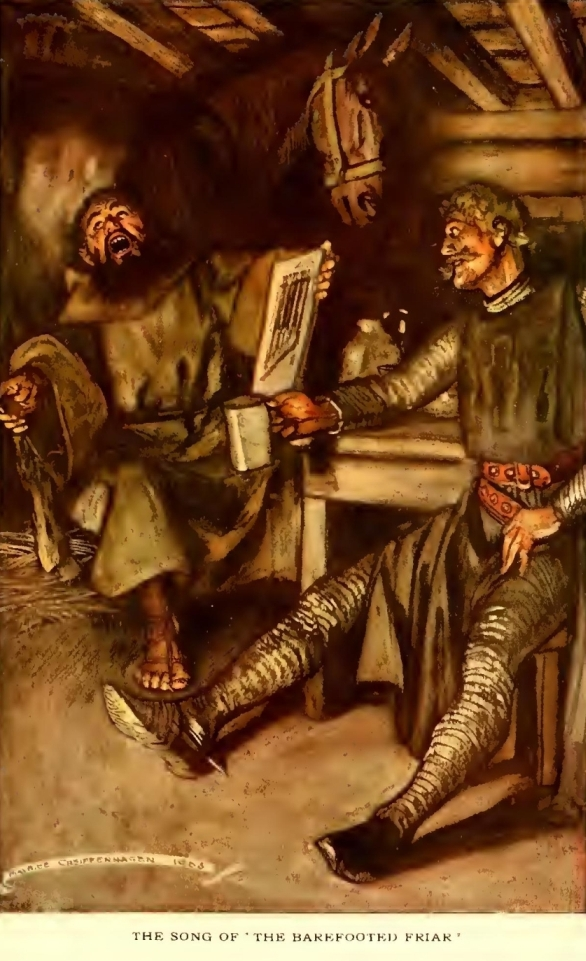
\includegraphics[height=.9\textheight]{ivanhoe/0239m}
    \caption{\scshape{the song of `the barefooted friar'.}}
\end{figure}

\begin{verse}
\versetitle{The Barefooted Friar.}

\flagverse{1.}
I'll give thee, good fellow, a twelvemonth or twain,\\
To search Europe through, from Byzantium to Spain;\\
But ne'er shall you find, should you search till you tire,\\
So happy a man as the Barefooted Friar.\\!
\flagverse{2.}
Your knight for his lady pricks forth in career,\\
And is brought home at even-song prick'd through with a spear;\\
I confess him in haste--for his lady desires\\
No comfort on earth save the Barefooted Friar's.\\!
\flagverse{3.}
Your monarch?--Pshaw! many a prince has been known\\
To barter his robes for our cowl and our gown,\\
But which of us e'er felt the idle desire\\
To exchange for a crown the grey hood of a Friar!\\!
\flagverse{4.}
The Friar has walk'd out, and where'er he has gone,\\
The land and its fatness is mark'd for his own;\\
He can roam where he lists, he can stop when he tires,\\
For every man's house is the Barefooted Friar's.\\!
\flagverse{5.}
He's expected at noon, and no wight till he comes\\
May profane the great chair, or the porridge of plums\\
For the best of the cheer, and the seat by the fire,\\
Is the undenied right of the Barefooted Friar.\\!
\flagverse{6.}
He's expected at night, and the pasty's made hot,\\
They broach the brown ale, and they fill the black pot,\\
And the goodwife would wish the goodman in the mire,\\
Ere he lack'd a soft pillow, the Barefooted Friar.\\!
\flagverse{7.}
Long flourish the sandal, the cord, and the cope,\\
The dread of the devil and trust of the Pope;\\
For to gather life's roses, unscathed by the briar,\\
Is granted alone to the Barefooted Friar.\\!
\end{verse}

``By my troth,'' said the knight, ``thou hast sung well and lustily, and
in high praise of thine order. And, talking of the devil, Holy Clerk,
are you not afraid that he may pay you a visit during some of your
uncanonical pastimes?''

``I uncanonical!'' answered the hermit; ``I scorn the charge--I scorn it
with my heels!--I serve the duty of my chapel duly and truly--Two masses
daily, morning and evening, primes, noons, and vespers, `aves, credos,
paters'---''

``Excepting moonlight nights, when the venison is in season,'' said his
guest.

``\,`Exceptis excipiendis'\,'' replied the hermit, ``as our old abbot
taught me to say, when impertinent laymen should ask me if I kept every
punctilio of mine order.''

``True, holy father,'' said the knight; ``but the devil is apt to keep
an eye on such exceptions; he goes about, thou knowest, like a roaring
lion.''

``Let him roar here if he dares,'' said the friar; ``a touch of my cord
will make him roar as loud as the tongs of St Dunstan himself did. I
never feared man, and I as little fear the devil and his imps. Saint
Dunstan, Saint Dubric, Saint Winibald, Saint Winifred, Saint Swibert,
Saint Willick, not forgetting Saint Thomas a Kent, and my own poor
merits to speed, I defy every devil of them, come cut and long
tail.--But to let you into a secret, I never speak upon such subjects,
my friend, until after morning vespers.''

He changed the conversation; fast and furious grew the mirth of the
parties, and many a song was exchanged betwixt them, when their revels
were interrupted by a loud knocking at the door of the hermitage.

The occasion of this interruption we can only explain by resuming the
adventures of another set of our characters; for, like old Ariosto, we
do not pique ourselves upon continuing uniformly to keep company with
any one personage of our drama.
